\appendix

\chapter{Appendix}

\section{Appendix to Chapter 1}
\label{appendix1}

\subsection{Relation between $g_{it}(\tau)$ and $\psi_{it}(\tau)$}

The relation between $g_{it}(\tau)$ and $\psi_{it}(\tau)$  is given by :
\begin{align} \label{gphi}
    g_{it}(\tau) &= \frac{F_{it}'(\tau)}{1-F_{it}(\tau)} \nonumber \\
    &= \psi_{it}(\tau) + \psi_{it}'(\tau)\tau.
\end{align}

\newtheorem*{proof1}{Proof}
\begin{proof1}
The last equation above can be computed with the first derivative of $\psi_{it}(\tau)$ with respect to time. Using Definition \ref{eq:psi} we have :
\begin{align*}
\psi_{it}'(\tau) &= \dfrac{u' v - u v'}{v^2} = \dfrac{\dfrac{F_{it}'(\tau)}{1-F_{it}(\tau)}\tau + \ln(1-F_{it}(\tau))}{\tau^2} \\
&= \dfrac{\dfrac{F_{it}'(\tau)}{1-F_{it}(\tau)}}{\tau} + \dfrac{\ln(1-F_{it}(\tau))}{\tau^2}\\
\Rightarrow \psi_{it}'(\tau) \tau &= \dfrac{F_{it}'(\tau)}{1-F_{it}(\tau)} + \dfrac{\ln(1-F_{it}(\tau))}{\tau}\\
\Rightarrow \dfrac{F_{it}'(\tau)}{1-F_{it}(\tau)} &= \psi_{it}(\tau) + \psi_{it}'(\tau) \tau.
\end{align*} \qed
\end{proof1}

\subsection{Computation of $\psi_{it}(\tau) \tau$}

The quantity $\psi_{it}(\tau) \tau$ that we are looking for is :
\begin{equation}
    \psi_{it}(\tau) \tau = \int_0^{\tau}g_{it}(s) ds.
\end{equation}

\newtheorem*{proof2}{Proof}
\begin{proof2}
Integrating by parts $\psi_{it}'(s) s$ between 0 and $\tau$, we have :
\begin{align*}
    \int_0^{\tau}\psi_{it}'(s)\cdot s \cdot ds &= \psi_{it}(s) \cdot s|_{s=0}^{s=\tau} - \int_0^{\tau}\psi_{it}(s) \cdot 1 \cdot ds \\
    &= \psi_{it}(\tau) \tau - \int_0^{\tau}\psi_{it}(s) ds.
\end{align*}
Integrating both sides of equation \ref{gphi} leads to :
\begin{align*}
    \int_0^{\tau} g_{it}(s) ds &= \int_0^{\tau}\psi_{it}(s)ds + \int_0^{\tau}\psi_{it}'(s)\cdot s \cdot ds \\
    &= \int_0^{\tau}\psi_{it}(s)ds + \psi_{it}(\tau) \tau - \int_0^{\tau}\psi_{it}(s) ds \\
    &= \psi_{it}(\tau) \tau.
\end{align*} \qed
\end{proof2}

\subsection{Likelihood function}


The likelihood function has been developed in \citet{Duan2012}. However, the likelihoods have to be slightly updated to be compatible with the neural network framework. One neural network is trained to compute $f_{it}$ and the other is trained to output $h_{it}$ where $g_{it} = f_{it} + h_{it}$.  Let us denote $\lambda$ and $\mu$ the set of parameters (weights) tuned in the neural network for $f_{it}$ and $h_{it}$ respectively. I impose non-negativity on both $f_{it}$ and $h_{it}$ to ensure that the combined exit intensity is at least bigger than the forward default intensity. The overall likelihood function for horizon of prediction $\tau$ is by definition given by 
\begin{equation} \label{biglik}
\mathcal{L}_\tau(\lambda,\mu; \tau_C,\tau_D, X) = \prod_{i=1}^N \prod_{t=0}^{T-1} \mathcal{L}_{\tau,i,t}(\lambda,\mu; \tau_{C_i},\tau_{D_i}, X_{it}),
\end{equation}
where
\begin{align}
    \mathcal{L}_{\tau,i,t}(\lambda,\mu; \tau_{C_i},\tau_{D_i}, X_{it}) &= \textbf{1}_{t_{0_i} \leq t, \tau_{C_i} > t+\tau+1} \cdot \mathbb{P}_t(\tau_{C_i} > t + \tau + 1) \\ \nonumber
    &+ \textbf{1}_{t_{0_i} \leq t, \tau_{D_i}=\tau_{C_i} \leq t+\tau} \cdot \mathbb{P}_t(t+\tau < \tau_{D_i} = \tau_{C_i} \leq t + \tau + 1) \\ \nonumber
    &+ \textbf{1}_{t_{0_i} \leq t, \tau_{C_i} \leq t+\tau, \tau_{D_i} \neq \tau_{C_i}} \cdot \mathbb{P}_t(t+\tau < \tau_{D_i} \neq \tau_{C_i} \leq t+\tau + 1) \\ \nonumber
    &+ \textbf{1}_{t_{0_i}>t} + \textbf{1}_{\tau_{C_i} \leq t},
\end{align}
with
\begin{align}
    \mathbb{P}_t(\tau_{C_i} > t + \tau + 1) &= \exp(-\sum_{s=0}^{\tau}g_{it}(s)\Delta t), \\
    \mathbb{P}_t(t+\tau < \tau_{D_i} = \tau_{C_i} \leq t + \tau + 1) &=    
    \begin{cases}
      1-\exp(-f_{it}(0)\Delta t), & \text{if}\ \tau_{C_i} = t+1 \\
      \exp(-\sum\limits_{s=0}^{\tau_{C_i}-t-2}g_{it}(s)\Delta t) \times \\
          \qquad (1-\exp[-f_{it}(\tau_{C_i}-t-1)\Delta t], & \text{otherwise}
    \end{cases} \\
    \mathbb{P}_t(t+\tau < \tau_{D_i} \neq \tau_{C_i} \leq t+\tau + 1)&=
    \begin{cases}
      1-\exp(-g_{it}(0)\Delta t)- \\ 
      \qquad ( 1-\exp(-f_{it}(0)\Delta t)), & \text{if}\ \tau_{C_i} = t+1 \\
      \exp(-\sum\limits_{s=0}^{\tau_{C_i}-t-2}g_{it}(s)\Delta t) \times \\
          \qquad (\exp[-f_{it}(\tau_{C_i}-t-1)\Delta t -  \\ 
          \qquad \exp[-g_{it}(\tau_{C_i}-t-1)\Delta t], & \text{otherwise}
    \end{cases}
\end{align}

Since the indicator functions are all mutually exclusive, taking the log of the likelihood function is very helpful. After the log-linearization, the product terms become summation terms, and the two last indicator functions drop. We are left with the summation of the indicator functions times the logarithm of each probability defined above. Similar to the proposition 2 in \citet{DSW} and subsection 3.2 in \citet{Duan2012}, the pseudo log-likelihood is the product of seperate terms which are function of $f$ and $g$. The first decomposition consists of separating terms involving $f$ and terms involving $g$. The second decomposition consists of separating terms corresponding to different $\tau$. In the end, we get two likelihood functions to estimate for each horizon. For each horizon the parameters of the likelihood function involving $f$ are estimated in a neural network with output $N_{it}^{(\lambda)}$. The parameters of the likelihood function involving $h$ are estimated in a neural network with output $N_{it}^{(\mu)}$. The combined exit forward intensity $g$ is assumed to be of the form $f + h$ as in previous literature. Since $\exp(-f)-\exp(-g) = \exp(-f)-\exp(-f-h) = \exp(-f)*(1-\exp(-h))$, the first decomposition is the following :
\begin{align}
    \mathcal{L}_{\tau,i,t}(\lambda; \tau_{C_i},\tau_{D_i}, X_{it}) &= \textbf{1}_{t_{0_i} \leq t, \tau_{C_i} > t+\tau+1} \cdot \exp(-\sum_{s=0}^{\tau} f_{it}(s)\Delta t) \\ \nonumber
    &+ \textbf{1}_{t_{0_i} \leq t, \tau_{D_i}=\tau_{C_i} \leq t+\tau} \cdot \exp(-\sum_{s=0}^{\tau_{C_i}-t-2} f_{it}(s)\Delta t) \cdot (1 - \exp(-f_{it}(\tau_{C_i}-t-1)\Delta t) \\ \nonumber
    &+ \textbf{1}_{t_{0_i} \leq t, \tau_{C_i} \leq t+\tau, \tau_{D_i} \neq \tau_{C_i}} \cdot \exp(-\sum_{s=0}^{\tau_{C_i}-t-2} f_{it}(s) \Delta t) \cdot \exp(-f_{it}(\tau_{C_i}-t-1)\Delta t) \\ \nonumber
    &+ \textbf{1}_{t_{0_i}>t} + \textbf{1}_{\tau_{C_i} \leq t},
\end{align}
\begin{align}
    \mathcal{L}_{\tau,i,t}(\mu; \tau_{C_i},\tau_{D_i}, X_{it}) &= \textbf{1}_{t_{0_i} \leq t, \tau_{C_i} > t+\tau+1} \cdot \exp(-\sum_{s=0}^{\tau} h_{it}(s)\Delta t) \\ \nonumber
    &+ \textbf{1}_{t_{0_i} \leq t, \tau_{D_i}=\tau_{C_i} \leq t+\tau} \cdot \exp(-\sum_{s=0}^{\tau_{C_i}-t-2} h_{it}(s)\Delta t)  \\ \nonumber
    &+ \textbf{1}_{t_{0_i} \leq t, \tau_{C_i} \leq t+\tau, \tau_{D_i} \neq \tau_{C_i}} \cdot \exp(-\sum_{s=0}^{\tau_{C_i}-t-2} h_{it}(s) \Delta t) \cdot (1-\exp(-h_{it}(\tau_{C_i}-t-1)) \\  \nonumber
    &+ \textbf{1}_{t_{0_i}>t} + \textbf{1}_{\tau_{C_i} \leq t}.
\end{align}
Similar to previous literature, we can still decompose the likelihoods into terms involving different horizons of prediction $\tau$. For each $\tau$, we can consider as constant all terms involving previous horizons forward intensities. After log-linearization, the second decomposition is the following :

\begin{align}
    \mathcal{L}_{i,t}(\lambda; \tau_{C_i},\tau_{D_i}, X_{it}) &= \textbf{1}_{t_{0_i} \leq t, \tau_{C_i} > t+\tau+1} \cdot (-f_{it}(s)\Delta t)) \\ \nonumber
    &+ \textbf{1}_{t_{0_i} \leq t, \tau_{D_i}=\tau_{C_i} \leq t+\tau}  \cdot \ln(1 - \exp(-f_{it}(s)\Delta t)) \\ \nonumber
    &+ \textbf{1}_{t_{0_i} \leq t, \tau_{C_i} \leq t+\tau, \tau_{D_i} \neq \tau_{C_i}} \cdot (-f_{it}(s)\Delta t),  \nonumber
\end{align}
\begin{align}
    \mathcal{L}_{i,t}(\mu; \tau_{C_i},\tau_{D_i}, X_{it}) &= \textbf{1}_{t_{0_i} \leq t, \tau_{C_i} > t+\tau+1} \cdot (- h_{it}(s)\Delta t) \\ \nonumber
    &+ \textbf{1}_{t_{0_i} \leq t, \tau_{C_i} \leq t+\tau, \tau_{D_i} \neq \tau_{C_i}} \cdot \ln(1-\exp(-h_{it}(s) \Delta t)). \\  \nonumber
\end{align}
For all horizon of prediction s. We are now left with many small likelihoods that we can maximize separately instead of the huge maximum likelihood \ref{biglik}. Ultimately, we can design two neural networks $NN_{\lambda}$ and $NN_{\mu}$ with outputs $N_{it}^{\lambda}$ and $N_{it}^{\mu}$ respectively to maximize the two above loss functions. 

\subsection{Distance-to-Default estimation}

\subsubsection{Distance-to-default}

Let $V_T$ be the firm value at time $T$, $L$ the amount of debt to be repaid and $E_T$ the equity value at time $T$. In case of bankruptcy, debt holders receive money before shareholders. The payoff to shareholders is then given by $E_T = \max(V_T - L,0)$. This payoff is the same as a call option $E_T$ on the underlying $V_T$ with the strike being $L$. \citet{Merton1974} model considers that $V_t$ is following a geometric Brownian motion :
\begin{equation*}
dV_t = \mu V_t d_t + \sigma V_t dB_t.
\end{equation*}
We can then use Black-Scholes formula to get the option price and firm's equity value $E_t$ at any time $t$ :
\begin{equation} \label{blackscholes}
E_t = V_t N(d_t) - e^{-r(T-t)}\cdot L \cdot N(d_t - \sigma \sqrt{T-t}),
\end{equation}
\begin{equation*}
d_t = \dfrac{\ln(V_t/L)+(r+\sigma^2/2)(T-t)}{\sigma \sqrt{T-t}},
\end{equation*}
with r being the risk-free rate and N(x) the normal cumulative distribution function.
The distance-to-default is defined as the difference between the expected value of the asset and the default point. After substitution into a normal cumulative distribution function, we get :
\begin{equation}
DtD_t = \dfrac{\ln(\dfrac{V_A}{L})+(\mu-\dfrac{\sigma_A^2}{2})(T-t)}{\sigma_A \sqrt{T-t}}.
\end{equation}
Note that similarly to the variance restriction method, $\mu$ cannot be estimated precisely. Thus, we compute DtD with the following formula :
\begin{equation}
DtD = \dfrac{\ln(\dfrac{V_A}{L})}{\sigma_A \sqrt{T-t}}.
\end{equation}
In Figure \ref{fig:DD} taken from \citet{KMV}, the distance-to-default is denoted by ``DD". The higher the asset value at horizon H the greater the distance-to-default will get, which lowers the default probability since the firm is more likely to be able to repay the debt owed. Similarly, the more debt the firm has, the smaller the DtD will be for a given level of asset value.

\begin{figure}[h!]
\centering
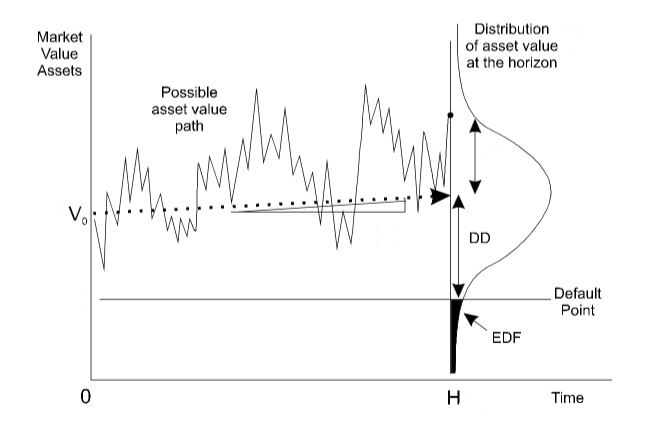
\includegraphics[width=0.75\textwidth]{DTD_Crosbie_Bohn.JPG} 
\mycaption{Distance-to-default}{The distance-to-default is denoted by DD. It is defined as the difference between the expected value of the asset and the default point. } 
\label{fig:DD}
\end{figure}



\subsubsection{Variance restriction method to estimate DtD}
The variance restriction method is used in \citet{DSW} to estimate the distance-to-default (DtD). This method is based on \citet{Merton1974} model which states that the firm's equity value can be seen as a call option on the underlying asset and the strike being the amount of debt. This holds because stockholders receive money only once debt holders are fully paid. \\
Applying the Black-Scholes call option formula to equity value, we get the following :
\begin{equation*}
\left\{
  \begin{array}{lll}
    V_E & = & V_A N(d_1) - e^{-r(T-t)} \cdot D \cdot N(d_2)\\
    d_1 & = & \dfrac{\dfrac{V_A}{D}+(r-\dfrac{\sigma_A^2}{2}(T-t)}{\sigma_A \sqrt{T-t}} \\
    d_2 & = & d_1 - \sigma_A \sqrt{T-t}.
  \end{array}
\right.
\end{equation*}
Where $V_E$ is the market equity value, $V_A$ is the market asset value, D is the default point and N the normal cumulative distribution function. Following KMV assumption, the default point D in the variance restriction method is specified as short-term debt plus one half of long-term debt.\\
Using It\^o, we can show that 
\begin{equation*}
\sigma_E = \dfrac{V_A}{V_E}\cdot \frac{\partial V_E}{\partial V_A}\cdot \sigma_A.
\end{equation*}
Hence, the method consists of solving the following system with two equations and two unknowns $V_A$ and $\sigma_A$ :
\begin{equation*}
\left\{
  \begin{array}{lll}
    V_E & = & V_A N(d_1) - e^{-r(T-t)} \cdot D \cdot N(d_2)\\
    \sigma_E & = & \dfrac{V_A}{V_E}\cdot \frac{\partial V_E}{\partial V_A}\cdot \sigma_A,
  \end{array}
\right.
\end{equation*}
Once $V_A$ and $\sigma_A$ are estimated, the DtD is defined as the distance between the expected value of the asset and the default point. After substitution in a normal CDF, we get
\begin{equation}
DtD = \dfrac{\ln(\dfrac{V_A}{L})+(\mu-\dfrac{\sigma_A^2}{2})(T-t)}{\sigma_A \sqrt{T-t}}.
\end{equation}
However, many papers agree that $\mu$ is very tedious to estimate. Hence, DtD is often computed as
\begin{equation}
DtD = \dfrac{\ln(\dfrac{V_A}{L})}{\sigma_A \sqrt{T-t}}.
\end{equation}

The major drawback of the variance restriction method used in \citet{DSW} is the definition of the default point. The default point in the variance restriction method is following the so-called KMV assumption. This assumption states that for every firm the default point is exactly equal to short term debt plus one half of long-term debt. However, many financial firms do not account debt as short or long-term debt but as ``other liabilities''. This causes the default point to be abnormally low for financial firms when using KMV assumption. Therefore, to take financial firms into account, we need to adjust the default point by taking into account other liabilities. The method proposed by \citet{Duan2012} employs a maximum likelihood to estimate the optimal fraction $\delta$ of other liabilities to include in the model.

\subsubsection{Maximum likelihood estimation to estimate DtD}

\citet{Duan2012} and \citet{Duan2012DTD} presented a method to estimate distance-to-defaults without having to exclude financial firms. The method accounts for other liabilities using a maximum likelihood estimation including a parameter $\delta$ to take into account other liabilities. 
The default point in this method becomes :
\begin{equation}
L = \text{short-term debt} + 0.5 \times \text{long-term debt} + \delta \times \text{other liabilities}.
\end{equation}
\citet{Duan2012} and \citet{Duan2012DTD} usually estimate $\delta$ for many firms altogether (i.e. $\delta$ for a whole industry). However, we improve the methodology by computing $\delta$ for each firm individually. We should obtain higher deltas for financial firms than for non-financial firms. Estimating $\delta$ for each firm is highly time consuming because of greater computation time but it should highly improve the granularity and precision of the model.
The log-likelihood function is given in \citet{Duan2012} and \citet{Duan2012DTD} by :
\begin{align*}
\mathcal{L}_i(\mu,\sigma,\delta) &= -\dfrac{n-1}{2}\ln(2\pi) - \dfrac{1}{2}\sum_{t=2}^n \ln(\sigma^2h_t) - \sum_{t=2}^n \ln(\dfrac{\hat{V}_t(\sigma,\delta)}{A_t}) \\
&-\sum_{t=2}^n \ln(N(\hat{d}_t(\sigma,\delta))) -\sum_{t=2}^n \dfrac{1}{2\sigma^2h_t} \times (\ln(\dfrac{\hat{V}_t(\sigma,\delta)}{\hat{V}_{t-1}(\sigma,\delta)}\cdot \dfrac{A_{t-1}}{A_t}-(\mu - \dfrac{\sigma^2}{2}))^2.
\end{align*}
where n is the number of period observations for each firm $i$. The likelihood above differs from \citet{Duan2012} and \citet{Duan2012DTD} because of the index $i$ since we estimate the likelihood for each of the 2099 firms in our sample to get 2099 estimations of $\delta$. Using this kind of likelihood is complex and very time consuming because we have to solve many inverse Black-Scholes formulas to get the time values of implied asset value $\hat{V}_t(\sigma,\delta)$ for each firm by solving equation \ref{blackscholes}. However, inverse Black-Scholes formula does not have any closed form solution. The optimization is even more tedious since the implied asset value $\hat{V}_t(\sigma,\delta)$ depends on the final output of the likelihood $\delta$. $A_t$ is the book asset value and $h_t$ is the time interval as a fraction of a year between two observations. $h_t$ in the model is set to be 0.25 since we performed a linear interpolation when we had a missing value in the sample (see ``Missing information"). To get rid of the inverse Black-Scholes formula problem, I use a dichotomic algorithm to compute the time series of asset values.\\



\section{Appendix to Chapter 2}
\label{appendix2}
\subsection{Technical proofs}
\subsubsection{Proof of Lemma \ref{lemma:small}}
From the definition of DIG, we know that for any $R_k\not\in\mathcal{PA}_j$, 
$
 I(R_k\rightarrow R_j||\mathcal{R}_{-\{k,j\}})=0   
$. 
This implies that for all $t$, 
\begin{align}\label{eq:app_l1}
     p(R_{j,t}|\mathcal{R}^{t-1})=p(R_{j,t}|\mathcal{R}_{-\{k\}}^{t-1}).
\end{align}
On the other hand, by the assumption of the Lemma, $R_i\not\in\mathcal{PA}_j$, we have
\begin{align}\label{eq:app_ll2}
 I(R_i\rightarrow R_j||\mathcal{R}_{-\{i,j\}})=0,  
\end{align}
or equivalently, for all $t$,
\begin{align}\label{eq:app_p1}
     p(R_{j,t}|\mathcal{R}^{t-1})=p(R_{j,t}|\mathcal{R}_{-\{i\}}^{t-1}).
\end{align}
 Combining \eqref{eq:app_l1} and \eqref{eq:app_p1} imply that for any pair $\{R_i,R_k\}$ that are not in the parent set of $R_j$, we have
\begin{align}\label{eq:app_l1_2}
   p(R_{j,t}|\mathcal{R}_{-\{k\}}^{t-1})=p(R_{j,t}|\mathcal{R}_{-\{i\}}^{t-1}).
\end{align}
To prove the claim of this lemma, we use \eqref{eq:app_l1_2} to show that all the time series in $\mathcal{R}_{-\{i,j\}}\setminus\mathcal{C}$ can be removed from the conditioning in \eqref{eq:app_ll2}. 
Let $R_k\in \mathcal{R}_{-\{i,j\}}\setminus\mathcal{C}$, by multiplying the above equality with $p(R_{i}^{t-1}|\mathcal{R}_{-\{i,k\}}^{t-1})$ and marginalizing over $R_{i}^{t-1}$, we obtain
\begin{align*}
    &\int p(R_{j,t}|\mathcal{R}_{-\{k\}}^{t-1})p(R_{i}^{t-1}|\mathcal{R}_{-\{i,k\}}^{t-1})dR_i^{t-1}=p(R_{j,t}|\mathcal{R}_{-\{i,k\}}^{t-1})\\
    &=\int p(R_{j,t}|\mathcal{R}_{-\{i\}}^{t-1})p(R_{i}^{t-1}|\mathcal{R}_{-\{i,k\}}^{t-1})dR_i^{t-1}=p(R_{j,t}|\mathcal{R}_{-\{i\}}^{t-1}).
\end{align*}
The above equalities and \eqref{eq:app_p1} imply that for all $t$,
\begin{align*}
p(R_{j,t}|\mathcal{R}^{t-1})=p(R_{j,t}|\mathcal{R}_{-\{i,k\}}^{t-1}),    
\end{align*}
or equivalently,  
\begin{align*}
    I(R_i\rightarrow R_j||\mathcal{R}_{-\{i,j,k\}})=0.
\end{align*}
By repeating the above procedure, we obtain
\begin{align*}
    I(R_i\rightarrow R_j||\mathcal{C})=0.
\end{align*}



\subsubsection{Proof of Lemma \ref{lemma:lin}}
Consider the VAR model in \eqref{eq:linearsys}. 
First, we assume that $X_i$ has no influence on $X_j$, i.e., $I(X_i\rightarrow X_j||\mathcal{X}_{-\{i,j\}})=0$ or equivalently $a_{j,i}=0$ and show that \eqref{eq:lemma_linear} holds. Given this assumption, we have that for all $t$,
\begin{align*}
    &p(X_{j,t}|\mathcal{X}_{-\{i\}}^{t-1})=p(X_{j,t}|\mathcal{X}^{t-1}).
\end{align*}
Using the equations in \eqref{eq:linearsys} and the assumption that $a_{j,i}=0$, we obtain
\begin{align*}
    &p(X_{j,t}|\mathcal{X}^{t-1})= p(N_{j,t}+\sum_{k}a_{j,k}X_{k,t-1}|\mathcal{X}^{t-1})=p(N_{j,t}+\sum_{k\neq i}a_{j,k}X_{k,t-1}|\mathcal{X}^{t-1})\\ 
    &=p(N_{j,t}+\sum_{k\neq i}a_{j,k}X_{k,t-1}|\sum_{k\neq i}a_{j,k}X_{k,t-1},{X}_{i}^{t-1},{X}_{j}^{t-1})\\
    &=p(N_{j,t}+\sum_{k\neq i}a_{j,k}X_{k,t-1}|\sum_{k\neq i}a_{j,k}X_{k,t-1},{X}_{j}^{t-1}).
\end{align*}
Note that we could replace $\mathcal{X}^{t-1}$ by $\{\sum_{k\neq i}a_{j,k}X_{k,t-1},{X}_{i}^{t-1},{X}_{j}^{t-1}\}$ or\\
$\{\sum_{k\neq i}a_{j,k}X_{k,t-1},{X}_{j}^{t-1}\}$ in the above equations, because given either of them $\sum_{k\neq i}a_{j,k}X_{k,t-1}$ becomes a constant and independent of $N_{j,t}$.
By defining $Q_{t-1}:=\sum_{k\neq i}a_{j,k}X_{k,t-1}$, the above equations can be rewritten as follows 
\begin{align*}
    &p(X_{j,t}|\mathcal{X}^{t-1})=p(X_{j,t}|Q_{t-1},{X}_{i}^{t-1},{X}_{j}^{t-1})=p(X_{j,t}|Q_{t-1},{X}_{j}^{t-1}), \forall t,
\end{align*}
or equivalently, 
\begin{align*}
    &\mathbb{E}\left[\log\frac{p(X_{j,t}|Q_{t-1},{X}_{i}^{t-1},{X}_{j}^{t-1})}{p(X_{j,t}|Q_{t-1},{X}_{j}^{t-1})}\right]=0, \forall t.
\end{align*}
Using the definition of DI, the above equalities can be written in terms of DI as follows
\begin{align*}
   I(X_i\rightarrow X_j||Q)=0.
\end{align*}
On the other hand, we have 
\begin{align*}
&[a_{j,1},...,a_{j,i-1},a_{j,i+1},...,a_{j,m}]=\arg\min_{\textbf{w}\in\mathbb{R}^{m-1}}\mathbb{E}\left[||X_{j,t}- \textbf{w}^T \textbf{X}_{-\{i\},t-1}||_2^2\right]:=\textbf{u}_t.
\end{align*}
where $\textbf{X}_{-\{i\},t-1} :=[X_{1,t-1},..., X_{i-1,t-1}, X_{i+1,t-1},..., X_{m,t-1} ]^T$. This means that $Q_{t-1}=\textbf{u}_t^T\textbf{X}_{-\{i\},t-1}$.

Next, we show the reverse direction, i.e.,  we assume \eqref{eq:lemma_linear} holds, then we show $I(X_i\rightarrow X_j||\mathcal{X}_{-\{i,j\}})=0$. To do so, it suffices to show $a_{j,i}=0$.
Since \eqref{eq:lemma_linear} holds, we have 
\begin{align*}
    {p(X_{j,t}|\textbf{u}_t^T\textbf{X}_{-\{i\},t-1},{X}_{i}^{t-1},{X}_{j}^{t-1})}={p(X_{j,t}|\textbf{u}_t^T\textbf{X}_{-\{i\},t-1},{X}_{j}^{t-1})}, \forall t.
\end{align*}
Using the $j$-th equation of \eqref{eq:linearsys} and the above equalities, for any instances $(\textbf{u}_t^T\textbf{x}_{-\{i\},t-1},{x}_{i}^{t-1},{x}_{j}^{t-1})$ of $(\textbf{u}_t^T\textbf{X}_{-\{i\},t-1},{X}_{i}^{t-1},{X}_{j}^{t-1})$, we obtain $\forall t$,
\begin{align*}
    &\mathbb{E}\left[{X_{j,t}|\textbf{u}_t^T\textbf{x}_{-\{i\},t-1},{x}_{i}^{t-1},{x}_{j}^{t-1}}\right]=\mathbb{E}\left[{X_{j,t}|\textbf{u}_t^T\textbf{x}_{-\{i\},t-1},{x}_{j}^{t-1}}\right],
\end{align*}
which implies
\begin{align*}
    &\mathbb{E}\left[N_{j,t}\right]+\sum_{k\neq i}a_{j,k}x_{k,t-1}+a_{j,i}x_{i,t-1}=\\
    &\mathbb{E}\left[N_{j,t}\right]+\sum_{k\neq i}a_{j,k}x_{k,t-1}
    +a_{j,i}\mathbb{E}\left[X_{i,t-1}|\textbf{u}_t^T\textbf{x}_{-\{i\},t-1},{x}_{j}^{t-1}\right].
\end{align*}
This simplifies to  
\begin{align*}
    a_{j,i}x_{i,t-1}=a_{j,i}\mathbb{E}\left[X_{i,t-1}|\textbf{u}_t^T\textbf{x}_{-\{i\},t-1},{x}_{j}^{t-1}\right], \forall t.
\end{align*}
This equation should hold for any $x_{i,t-1}$. This is only possible if $a_{j,i}=0$.





\subsubsection{Proof of Lemma \ref{lemma:nonlinear}}
The proof is similar to the linear version and uses the fact that exogenous noises $\{\varepsilon_{j,t}\}$ are independent. More precisely, we have  
\begin{align*}
    &p(X_{j,t}|\mathcal{X}^{t-1})=p(F_{j}(\mathcal{X}^{t-1}) + \varepsilon_{j,t}|F_{j}(\mathcal{X}^{t-1})).
\end{align*}
Since there is no influence from $X_i$ to $X_j$, we can eliminate it from the conditioning and the argument of function $F_j$ and obtain
\begin{align*}
&p\big(F_{j}(\mathcal{X}^{t-1}) + \varepsilon_{j,t}|\mathcal{X}^{t-1}\big)=p\big(F_{j}(\mathcal{X}_{-\{i\}}^{t-1}) + \varepsilon_{j,t}|\mathcal{X}_{-\{i\}}^{t-1}\big).
\end{align*}
On the other hand, because given either $\{F_{j}(\mathcal{X}_{-\{i\}}^{t-1}), X_i^{t-1},X_j^{t-1}\}$ or \\
$\{F_{j}(\mathcal{X}_{-\{i\}}^{t-1}),X_j^{t-1}\}$, the value of $F_{j}(\mathcal{X}_{-\{i\}}^{t-1})$ is no longer a random variable. Using this relationship and the fact that $\varepsilon_{j,t}$ is independent of $\mathcal{X}^{t-1}$, we obtain
\begin{small}
\begin{align*}
    &p\big(F_{j}(\mathcal{X}_{-\{i\}}^{t-1}) + \varepsilon_{j,t}|F_{j}(\mathcal{X}_{-\{i\}}^{t-1}), X_i^{t-1},X_j^{t-1}\big)=
    p\big(F_{j}(\mathcal{X}_{-\{i\}}^{t-1}) + \varepsilon_{j,t}|F_{j}(\mathcal{X}_{-\{i\}}^{t-1}), X_j^{t-1}\big).
\end{align*}
\end{small}
By defining $Q_{t-1}:=F_{j}(\mathcal{X}_{-\{i\}}^{t-1})$, the above equations can be rewritten in terms of DI as follows,
\begin{align*}
    I(X_i\rightarrow X_j||Q)=0.
\end{align*}

To show the reverse, we need to prove that $I(X_i\rightarrow X_j||\mathcal{X}_{-\{i,j\}})=0$ if Equation \eqref{eq:non-q} holds.
Because $I(X_i\rightarrow X_j||Q)=0$ and using Equation \eqref{nonlinear}, for all $t$, we have
\begin{align*}
    &p\big(F_{j}(\mathcal{X}^{t-1}) + \varepsilon_{j,t}|Q_{t-1}, X_i^{t-1},X_j^{t-1}\big)=
    p\big(F_{j}(\mathcal{X}^{t-1}) + \varepsilon_{j,t}|Q_{t-1}, X_j^{t-1}\big),
\end{align*}
where $Q_{t-1}=F_{j}(\mathcal{X}_{-\{i\}}^{t-1})$. Note that the conditioning on the right-hand-side distribution is independent of $X_{i}^{t-1}$. This implies that function $F_j$ does not depend on $X_i$. Therefore, we can remove $X_i^{t-1}$ from the argument of $F_j$, i.e., 
\begin{align*}
    X_{j,t}=F_{j}(\mathcal{X}^{t-1})+\varepsilon_{j,t}=F_{j}(\mathcal{X}_{-\{i\}}^{t-1})+\varepsilon_{j,t},
\end{align*} 
which further implies
\begin{align*}
    &p(F_{j}(\mathcal{X}_{-\{i\}}^{t-1}) + \varepsilon_{j,t}|\mathcal{X}_{-\{i,j\}}^{t-1}, X_i^{t-1},X_j^{t-1})=
    p(F_{j}(\mathcal{X}_{-\{i\}}^{t-1}) + \varepsilon_{j,t}|\mathcal{X}_{-\{i,j\}}^{t-1},X_j^{t-1}). 
\end{align*}
This is equivalent to 
\begin{align*}
    I(X_i\rightarrow X_j||\mathcal{X}_{-\{i,j\}})=0.
\end{align*}


\begin{comment}
\subsection{k-Nearest Neighbors estimator of mutual information}
Suppose that $N+M$ i.i.d. realizations $\{\textbf{x}_1, ..., \textbf{x}_{N+M}\}$ are available from $\PP_{X,Y,Z}$, where $\textbf{x}_i$ denotes the $i$-th realization of $(X,Y,Z)$.
The data is randomly divided into two subsets $\mathcal{S}_1$ and $\mathcal{S}_2$ of $N$ and $M$ points, respectively.  
The estimator has two main stages:
In the first stage, a k-nearest density estimator $\widehat{\PP}_{X,Y,Z}$ at the $N$ points of $\mathcal{S}_1$ is estimated using the $M$ realizations of $\mathcal{S}_2$ as follows: 

Let $d(\textbf{x},\textbf{y})\in\mathbb{R}$ denote the Euclidean distance between points $\textbf{x}$ and $\textbf{y}$ and $d_k(\textbf{x})\in\mathbb{R}$ denotes the Euclidean distance between a point $\textbf{x}$ and its k-th nearest neighbor among
$\mathcal{S}_2$. The k-nearest region is $\mathcal{S}_k(\textbf{x}) := \{\textbf{y} :d(\textbf{x},\textbf{y})\leq d_k(\textbf{x}) \}$ and the volume of this region is $V_k(\textbf{x}):=\int_{\mathcal{S}_k(\textbf{x})}1dv$. The standard k-nearest density estimator of \cite{sricharan2011k} is defined as 
\begin{small}
\begin{align*}
&\widehat{\PP}_{X,Y,Z}(\textbf{x}):=\frac{k-1}{M\cdot V_k(\textbf{x})}.
\end{align*}
\end{small}
\noindent Similarly, we obtain k-nearest density estimators $\widehat{\PP}_{X,Z}, \widehat{\PP}_{Y,Z}$, and $\widehat{\PP}_{Z}$.
Subsequently, the $N$ samples of $\mathcal{S}_1$ is used to approximate the conditional mutual information:
\begin{small}
\begin{align*}
&\widehat{I}(X;Y|Z):=\frac{1}{N}\sum_{i\in \mathcal{S}_1} \log \widehat{\PP}_{X,Y,Z}(\textbf{x}_i) + \log \widehat{\PP}_{Z}(\textbf{x}_i) -\log \widehat{\PP}_{X,Z}(\textbf{x}_i) -\log \widehat{\PP}_{Y,Z}(\textbf{x}_i).
\end{align*}
\end{small}
\noindent For more details corresponding this estimator including its bias, variance, and confidence, please see the works by \cite{sricharan2011k} and \cite{loftsgaarden1965nonparametric}.
\end{comment}

\subsection{Koopman-based Lifting Method}
Let $\textbf{X}_t:=\{X_{1,t}, ..., X_{m,t}\}$ denote a network of $m$ time series such that 
\begin{align}\label{dyn}
\dot{\textbf{X}}_t = F(\textbf{X}_t),
\end{align}
where the vector field $F(\textbf{X})=(F_1(\textbf{X}),...,F_m(\textbf{X}))$ is of the form
\begin{align}
F_j(\textbf{X})= \sum_{k=1}^K w_{j,k} h_k(\textbf{X}).
\end{align}
In the above equation, $w_{j,k}\in\mathbb{R}$ are unknown weights and $\{h_k(\textbf{X})\}$ denote a set of known library functions, e.g., monomials. 
Furthermore, let $\varphi^t(\textbf{X}_0)$ denote the solution to \eqref{dyn} associated with the initial condition $\textbf{X}_0$. 

Now, suppose that we have $N$ noisy observations $\{(\textbf{x}_1, \textbf{y}_1), ..., (\textbf{x}_N, \textbf{y}_N)\}$ of the system trajectory, where $\textbf{x}_i$ is the initial point and $\textbf{y}_i$ is the final point after $T_s$ steps, i.e., 
\begin{align*}
\textbf{y}_i - \epsilon_i = \varphi^{T_s}(\textbf{x}_i - \varepsilon_i), \ \  i=1,...,N,
\end{align*}
where $\epsilon_i$ and $\varepsilon_i$ are the measurement noises. 
The goal is to estimate the weights $\{w_{j,k}\}$ using these observations and consequently infer the causal network among the time series. To do so, we use the Koopman approach \cite{mauroy2019koopman} that lifts the observation space to another space in which the relationships are linear. 
More precisely, the steps are as follows:
\begin{itemize}
\item Select a set of $M$ basis lifting functions $\{p_1(\textbf{x}), ..., p_M(\textbf{x})\}$, and lift the observations,
\begin{align}
\textbf{P}_x:=\begin{pmatrix}
p_1(\textbf{x}_1) & \cdots & p_M(\textbf{x}_1)\\
p_1(\textbf{x}_2) & \cdots & p_M(\textbf{x}_2)\\
\vdots  &  \ddots & \vdots  \\
p_1(\textbf{x}_N) & \cdots & p_M(\textbf{x}_N)
\end{pmatrix}, 
\textbf{P}_y:=\begin{pmatrix}
p_1(\textbf{y}_1) & \cdots & p_M(\textbf{y}_1)\\
p_1(\textbf{y}_2) & \cdots & p_M(\textbf{y}_2)\\
\vdots  &  \ddots & \vdots  \\
p_1(\textbf{y}_N) & \cdots & p_M(\textbf{y}_N)
\end{pmatrix}\!.
\end{align}

\item Identify the Koopman operator $\textbf{L}:=\frac{1}{T_s}\log(\textbf{P}_x^{\dagger}\textbf{P}_y)$, where $\textbf{P}_x^{\dagger}$ denotes the pseudo-inverse of $\textbf{P}_x$ and the function log denotes the (principal) matrix logarithm.



\item Identify the weights using the following equations: $\widehat{w}_{k,j}:=[\textbf{L}]_{k,l}$, with $l$ such that $p_l(\textbf{x})=x_j$, where $\textbf{x}=(x_1,...,x_m)$.

\end{itemize}

An alternative approach to obtain the weights is the dual lifting method which executes the following steps instead of the above last step.
%Consider the dynamic in \eqref{dyn} in which $F(X)=(F_1(X),...,F_n(X))$, and 
%\begin{align}\label{dy}
%F_j(X) = \sum_{k=1}^K w_{j,k} h_k(X).
%\end{align}
%The goal is to infer the weights $\{w_{j,k}\}$, when the library functions $\{h_k\}$ are assumed to be known.
%In order to present the steps of the Koopman method, we first represent the observational data $X_1,...,X_T$, where $T:=sT_0$ in  the following form. 
%\begin{align}
%D=\begin{pmatrix}
%X_1 & \cdots & X_{T_0}\\
%X_{T_0+1}& \cdots & X_{2T_0}\\
%\vdots  &  \ddots & \vdots  \\
%X_{(s-1)T_0+1} & \cdots & X_{sT_0}
%\end{pmatrix}_{s\times T_0}.
%\end{align}
%The steps of the Koopman method in this case is presented below. 
%\\
%\textbf{Note:} The basis functions $\{g_k\}$ can be monomials or Gaussian ($g_k(x)=\exp(-\gamma||x-x_k||)$). 
%\begin{algorithmic}[H]
%\STATE - Input: $\{(X_1,X_{T_0}), (X_{T_0+1},X_{2T_0}), ..., (X_{(s-1)T_0+1},X_{sT_0})\}$, bases
%\STATE   functions $\{g_1,...,g_M\}$, library functions $\{h_1,...,h_K\}$
%\STATE - Construct the following matrices
%\begin{align*}
%P_x:=\begin{pmatrix}
%g_1(X_1) & \cdots & g_M(X_1)\\
%g_1(X_{T_0+1}) & \cdots & g_M(X_{T_0+1})\\
%\vdots  &  \ddots & \vdots  \\
%g_1(X_{(s-1)T_0+1}) & \cdots & g_M(X_{(s-1)T_0+1})
%\end{pmatrix}_{s\times M},
%\end{align*}
%\begin{align*}
%P_y:=\begin{pmatrix}
%g_1(X_{T_0}) & \cdots & g_M(X_{T_0})\\
%g_1(X_{2T_0}) & \cdots & g_M(X_{2T_0})\\
%\vdots  &  \ddots & \vdots  \\
%g_1(X_{sT_0}) & \cdots & g_M(X_{sT_0})
%\end{pmatrix}_{s\times M}.
%\end{align*}
%\STATE - Compute the Koopman operator 
%$
%\widetilde{L}_{s\times s}:=\frac{1}{T_0}\log\left(P_yP_x^{\dagger}\right)
%$.
At first, it finds matrix $\widehat{\textbf{F}}$ using the following equation, 
\begin{align*}
\widehat{\textbf{F}}_{N\times m}:=
%\begin{pmatrix}
%\widehat{F}(X_1)^T \\
%\widehat{F}(X_{T_0+1})^T\\
%\vdots  \\
%\widehat{F}(X_{(s-1)T_0+1})^T
%\end{pmatrix}_{s\times n} 
\textbf{L}_{N\times N} \begin{pmatrix}
\textbf{x}^T_1 \\
\vdots  \\
\textbf{x}^T_{N} 
\end{pmatrix}_{N\times m}.
\end{align*}
Next, it constructs  
\begin{align*}
\textbf{H}_x:=\begin{pmatrix}
p_1(\textbf{x}_{1}) & \cdots & p_M(\textbf{x}_{1})\\
\vdots  &  \ddots & \vdots  \\
p_1(\textbf{x}_{N}) & \cdots & p_M(\textbf{x}_{N})
\end{pmatrix}_{N\times M},
\end{align*}
 and for each $j$, solve the following regression problem to get the weights
\begin{align*}
\widehat{\textbf{w}}_j :=\arg\min_{\textbf{w}\in\mathbb{R}^M}\left|\left|\textbf{H}_x \textbf{w} - \widehat{\textbf{F}}_{:,j} \right|\right|_2^2 + \rho ||\textbf{w}||_1,
\end{align*}
where $\widehat{\textbf{F}}_{:,j}$ denotes the $j$-th column of matrix $\widehat{\textbf{F}}$  and $\widehat{\textbf{w}}_j =[\hat{w}_{j,1}, ..., \hat{w}_{j,M}]^T$.
%\end{algorithmic}
% The last step of the algorithm is due to Equation \eqref{dy}.
% \begin{align*}
% \widehat{F}_j(X) := \sum_{k=1}^K \hat{w}_j^k h_k(X).
% \end{align*}

\subsection{Ideal portfolio}
In this section, we show how the ideal portfolio is related to the coefficients of the linear system in \eqref{eq:linearsys}.  
Recall the optimization problem in Lemma \ref{lemma:lin}. 
\begin{align*}
&\textbf{u}_t:=\arg\min_{\textbf{w}\in\mathbb{R}^{m-1}}\mathbb{E}\left[||X_{j,t}- \textbf{w}^T \textbf{X}_{-\{i\},t-1}||_2^2\right],\\
&\textbf{X}_{-\{i\},t-1} :=[X_{1,t-1},\cdots, X_{i-1,t-1}, X_{i+1,t-1}, \cdots, X_{m,t-1} ]^T.
\end{align*}
Consider the $j$-th Equation in \eqref{eq:linearsys}, i.e., 
\begin{align*}
    X_{j,t}=\sum_{k=1}^m a_{j,k}X_{k,t-1}+N_{j,t}.
\end{align*}
If $a_{j,i}=0$, by substituting the above equation into the optimization, we obtain
\begin{align*}
&\min_{\textbf{w}\in\mathbb{R}^{m-1}}\mathbb{E}\left[||\sum_{k\neq i} (a_{j,k}-w_{k})X_{k,t-1}+N_{j,t}||_2^2\right]=\min_{\textbf{w}\in\mathbb{R}^{m-1}}\mathbb{E}\left[||N_{j,t}||_2^2\right]\\
&+\mathbb{E}\left[||\sum_{k\neq i} (a_{j,k}-w_{k})X_{k,t-1}||_2^2\right]+2\mathbb{E}\left[||\left(\sum_{k\neq i} (a_{j,k}-w_{k})X_{k,t-1}\right)N_{j,t}||_2^2\right]\\
&=\min_{\textbf{w}\in\mathbb{R}^{m-1}}\mathbb{E}\left[||\sum_{k\neq i} (a_{j,k}-w_{k})X_{k,t-1}||_2^2\right]+\mathbb{E}\left[||N_{j,t}||_2^2\right]
\end{align*}
The last equality is due to the fact $N_{j,t}$ is independent of $\{X_{k,t-1}\}$ and have zero mean. This implies that the solution is $w_k=a_{j,k}$ for $k\in\{1,...,i-1,i+1,...,m\}$.











\begin{comment}
\subsection*{Appendix D : Ideal portfolio}
In this section, we present the relation between the ideal portfolio defined in Lemma \ref{lemma:lin} and maximally correlated portfolio. 
We use the following notations and definitions,
\begin{itemize}
\item $r$ denotes the risk-free return (random, but known at beginning of period),
  %\item $X_j$ denotes the excess return of stock $j$ over risk-free $r$,
  \item Candidate excess returns $\textbf{R}=(R_1,\dots,R_{m-1})^T$ over risk-free $r$,
  %(all stocks but $i$ and $j$, e.g., $m=498$)
  \item Covariance matrix of $\begin{pmatrix}
    X \\ \textbf{R}
  \end{pmatrix}$ is denoted by $\mathbf{\Sigma}:=\begin{pmatrix}
    \mathbf{\Sigma}_{XX} & \mathbf{\Sigma}_{X\textbf{R}} \\ \mathbf{\Sigma}_{\textbf{R}X} & \mathbf{\Sigma}_{\textbf{RR}}
  \end{pmatrix}  $. We assume that $\mathbf{\Sigma}_{\textbf{RR}}$ is invertible.
  
  \item Portfolio with relative weights $\textbf{w} \in \mathbb{R}^{m-1}$ has excess return over $r$ of
\[ Z(\textbf{w}) := \underbrace{\textbf{w}^T  (\textbf{R}+\textbf{1} r)+ (1-\textbf{w}^T \textbf{1}) r}_{\text{portfolio return}}  - r = \textbf{w}^T \textbf{R}.\]
\end{itemize}

Given the above definitions, the correlation of $Z(w)$ with $X$ will be
\begin{align}\label{eqcorr}
  corr(Z(\textbf{w}),X)\!\! &:=\! \dfrac{cov(Z(\textbf{w}),X)}{\sqrt{var(Z(\textbf{w}))var(X)}} = \dfrac{\mathbb{E}[(Z(\textbf{w})-\mathbb{E}[Z(\textbf{w})])^T(X-\mathbb{E}[X])]}{\sqrt{var(Z(\textbf{w}))var(X)}}\\
  &= \dfrac{\textbf{w}^T \mathbf{\Sigma}_{\textbf{R}X}}{\sqrt{\textbf{w}^T\mathbf{\Sigma}_{\textbf{RR}}\textbf{w}}\sqrt{\mathbf{\Sigma}_{XX}}}.
\end{align}
Note that this correlation is invariant under scaling the portfolio weights $w$:
\begin{equation}\label{eqt}
  corr(Z(\textbf{w}),X) = corr(Z(t \textbf{w}),X) \quad \text{for any $t>0$.}
\end{equation}
We can thus assume that $\textbf{w}$ is normalized, $\textbf{w}^T\mathbf{\Sigma}_{\textbf{RR}}\textbf{w}=1$.

Suppose that the goal is to find the portfolio $Z(\textbf{w})$ with normalized weights such that it is maximally correlated with $X$, i.e., 
%\begin{equation}\label{p0}
% \max_{w\in \mathbb{R}^m}  corr(Z(\textbf{w}),X).
% \end{equation}
%In view of \eqref{eqcorr} and \eqref{eqt}, problem \eqref{p0} is equivalent to the constraint optimization problem
\begin{equation}\label{p1}
\begin{aligned}
 \max_{\textbf{w}\in\mathbb{R}^{m-1}}\, &   corr(Z(\textbf{w}),X)   \\
 \text{subject to } &\textbf{w}^T\mathbf{\Sigma}_{\textbf{RR}}\textbf{w}=1,
\end{aligned}
 \end{equation}
 then the solution can be characterize analytically as follows. 

\begin{lemma}\label{lemw1}
The problem in \eqref{p1} has a unique solution and it is given by
\begin{align}\label{w1eq}
  {\textbf{w}^*} := \frac{\mathbf{\Sigma}_{\textbf{RR}}^{-1} \mathbf{\Sigma}_{\textbf{R}X}}{\sqrt{\mathbf{\Sigma}_{X\textbf{R}}\mathbf{\Sigma}_{\textbf{RR}}^{-1}\mathbf{\Sigma}_{\textbf{R}X}}}.
\end{align}
\end{lemma}
\begin{proof}
The Lagrangian to \eqref{p1} is
\[ L(\textbf{w},\mu) = \textbf{w}^T \mathbf{\Sigma}_{\textbf{R}X} - \mu( \textbf{w}^T\mathbf{\Sigma}_{\textbf{RR}}\textbf{w}-1)\]
for the Lagrangian multiplier $\mu\in\mathbb{R}$. The first order condition in $\textbf{w}$ reads $2\mu\mathbf{\Sigma}_{\textbf{RR}} \textbf{w}^* = \mathbf{\Sigma}_{\textbf{R}X}$, which yields
\[  \textbf{w}^* = \frac{1}{2\mu} \mathbf{\Sigma}_{\textbf{RR}}^{-1}\mathbf{\Sigma}_{\textbf{R}X}.\]
Choosing $\mu$ such that $\textbf{w}^{*T}\mathbf{\Sigma}_{\textbf{RR}}\textbf{w}^*=1$ gives
\[ 2\mu = \sqrt{\mathbf{\Sigma}_{X\textbf{R}}\mathbf{\Sigma}_{\textbf{RR}}^{-1} \mathbf{\Sigma}_{\textbf{RR}}\mathbf{\Sigma}_{\textbf{RR}}^{-1}\mathbf{\Sigma}_{\textbf{R}X}} =\sqrt{\mathbf{\Sigma}_{X\textbf{R}}\mathbf{\Sigma}_{\textbf{RR}}^{-1}\mathbf{\Sigma}_{\textbf{R}X}},\]
which proves \eqref{w1eq}.
\end{proof}

\paragraph{Relation with Ideal Portfolio:}
Recall the optimization problem in Lemma \ref{lemma:lin}. 
Herein, we rewrite it by substituting $X_{j,t}$ and $\textbf{X}_{-\{i\},t-1}$ by $X$ and $\textbf{R}$, respectively. 
\begin{align*}
&\min_{\textbf{w}\in\mathbb{R}^{m-1}}\mathbb{E}\left[||X- \textbf{w}^T \textbf{R}||_2^2\right].
\end{align*}
Note that this formulation is also related to the projection problem in which the goal is to project $X$ onto the space generated by $\textbf{R}$.
Without loss of generality, we assume that both $X$ and $\textbf{R}$ have zero means. This yields the following solution
\begin{align}\label{w2eq}
    \textbf{w}^{**}:=\mathbf{\Sigma}_{\textbf{RR}}^{-1} \mathbf{\Sigma}_{\textbf{R}X}.
\end{align}
Comparing \eqref{w1eq} and \eqref{w2eq} shows that the only difference is a normalization factor. Therefore, the maximally correlated portfolio contains the same information as the ideal portfolio. 

\paragraph{Maximal information in Gaussian case:}
In the case that the joint distribution is Gaussian, the maximally correlated (equivalently, ideal) portfolio $\textbf{w}^{*T} \textbf{R}$ ($\textbf{w}^{**T} \textbf{R}$) captures the same information about $X$ as the entire vector $\textbf{R}$ does, in the following sense.
\begin{lemma}
Assume that $(X,\textbf{R})$ is jointly Gaussian. Then the conditional variances of $X$ given the observation of all excess returns $\textbf{R}$ and of the maximally correlated (ideal) portfolio are the same, i.e., 
\begin{equation}\label{vareqXR}
  var(X\mid \textbf{R} ) = var(X\mid {\textbf{w}^*}^T \textbf{R} )= var(X\mid {\textbf{w}^{**}}^T \textbf{R} ).
\end{equation}
\end{lemma}
\begin{proof}
Gaussian conditioning gives
\[ var(X\mid \textbf{R} ) =\mathbf{\Sigma}_{XX} - \mathbf{\Sigma}_{X\textbf{R}}\mathbf{\Sigma}_{\textbf{RR}}^{-1}\mathbf{\Sigma}_{\textbf{R}X}, \]
and on the other hand
\begin{align*}
    var(X\mid {\textbf{w}^*}^T \textbf{R} ) &= \Sigma_{XX} - \mathbf{\Sigma}_{X\textbf{R}}{\textbf{w}^*}({\textbf{w}^*}^T\mathbf{\Sigma}_{\textbf{RR}}{\textbf{w}^*})^{-1}{\textbf{w}^*}^T\mathbf{\Sigma}_{\textbf{R}X} \\
    &= \Sigma_{XX} - \mathbf{\Sigma}_{X\textbf{R}}{\textbf{w}^*}{\textbf{w}^*}^T\mathbf{\Sigma}_{\textbf{R}X}\\
    &= \Sigma_{XX} - \mathbf{\Sigma}_{X\textbf{R}}\mathbf{\Sigma}_{\textbf{RR}}^{-1}\mathbf{\Sigma}_{\textbf{R}X}.
\end{align*}
Similarly, we have 
\begin{align*}
    &var(X\mid {\textbf{w}^{**}}^T \textbf{R} ) = \Sigma_{XX} - \mathbf{\Sigma}_{X\textbf{R}} {\textbf{w}^{**}}^T({\textbf{w}^*}^T\mathbf{\Sigma}_{\textbf{RR}} {\textbf{w}^{**}}^T)^{-1} {\textbf{w}^{**}}^T\mathbf{\Sigma}_{\textbf{R}X} \\
    &= \Sigma_{XX} - \mathbf{\Sigma}_{X\textbf{R}}\mathbf{\Sigma}_{\textbf{RR}}^{-1}\mathbf{\Sigma}_{\textbf{R}X}\big(\mathbf{\Sigma}_{X\textbf{R}}\mathbf{\Sigma}_{\textbf{RR}}^{-1}\mathbf{\Sigma}_{\textbf{R}X}\big)^{-1}\mathbf{\Sigma}_{X\textbf{R}}\mathbf{\Sigma}_{\textbf{RR}}^{-1}\mathbf{\Sigma}_{\textbf{R}X}\\
    &= \Sigma_{XX} - \mathbf{\Sigma}_{X\textbf{R}}\mathbf{\Sigma}_{\textbf{RR}}^{-1}\mathbf{\Sigma}_{\textbf{R}X}.
\end{align*}
\end{proof}

\begin{remark}
Equality \eqref{vareqXR} is not true in general for non-Gaussian $(X,\textbf{R})$. In particular, using \cite{din_16}, one can check that \eqref{vareqXR} does not hold for multivariate $t$-distributions.
\end{remark}


\end{comment}



\newpage 

\section{Appendix to Chapter 3}

\subsection{Tutorial for StockTwits Messages Extraction}\label{app_tut}

We use stock price data from CRSP/Compustat of all US and Canadian listed stocks from January 2010 to March 2020. From this dataset, we create the list of unique tickers for which we will extract messages. We will later be able to merge the two datasets using the date and ticker for every observation. We use the StockTwits Application Programming Interface (API) to download messages from StockTwits. One query on StockTwits API is called a JavaScript Object Notation (JSON) request. Every message on StockTwits has a unique identifier ("msg\_id") posted by a user with a unique identifier ("user\_id"). JSON requests allow to query the database by ticker (called "symbol method") or by user (called "user method"). We use the query by ticker. One query only outputs the latest 30 messages concerning that ticker. However, it is possible to set a parameter ("max") to output the latest 30 messages up to this particular message identifier. This parameter allows us to crawl the message history of a ticker by recursively changing the "max" parameter to the oldest message identifier in the query. To perform a JSON request for Apple (AAPL) up to the message identifier 30'000'000, simply enter the following URL in a browser : \url{https://api.stocktwits.com/api/2/streams/symbol/AAPL.json?\&max=30000000}. The page we get looks unreadable but it has always the same structure : several pairs of keys and values. The structure of JSON can easily be interpreted by modern programming languages. We create a Python script to query the API and extract the message history of every ticker in the ticker list. We store the output of every JSON request in .txt files in dedicated ticker folders.



\subsection{Message Count}\label{app_counting}

A StockTwits message can refer to multiple tickers. Figure \ref{fig:tickerpermessage} shows the histogram of the number of tickers tagged per message. As the vast majority of message includes only one ticker, we only show on this plot messages referring to more than one ticker. The maximum number of tickers per message amounts to 28 and corresponds to 11 messages in the sample. Many messages refer to several tickers and this creates duplicates in the database because we consider the same message for all tickers tagged in the message. 


\begin{figure}[h]
    \centering
    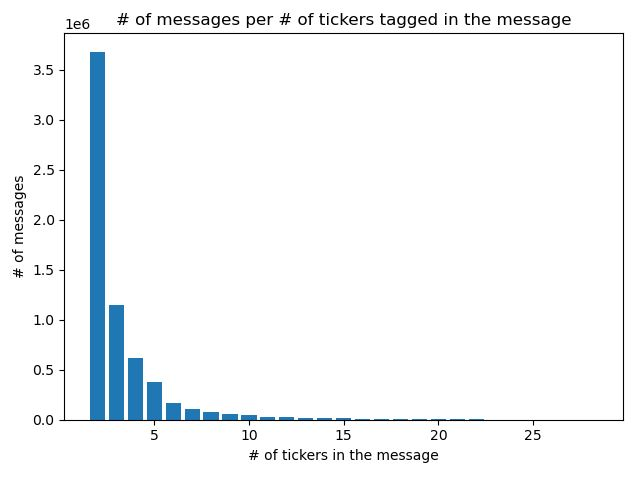
\includegraphics[width=0.75\textwidth]{hist_tic.jpg}
    \mycaption{Histogram of the number of tickers per message}{Histogram of the number of tickers per message, across all messages referring to more than one ticker.}
    \label{fig:tickerpermessage}
\end{figure}

Left plot of Figure \ref{fig:messagecount} shows the number of messages with and without double counting. In our sample, the number of messages without double counting is 76 million, as opposed to 90 million messages with double counting. Right plot of Figure \ref{fig:messagecount} shows the ratio between the number of messages with double counting and the number of messages without double counting. Throughout this paper, we only refer to the number of messages with double counting.



\begin{figure*}[h!]
\centering
        \begin{subfigure}{0.49\textwidth}   
            \centering 
            \includegraphics[width=\textwidth]{uniq.jpg}
        \end{subfigure}
        \begin{subfigure}{0.49\textwidth}   
            \centering 
            \includegraphics[width=\textwidth]{ratio.jpg}
        \end{subfigure}
        \mycaption{Number of messages}{Left plot shows the total number of messages with double counting (red) compared to the total number of messages without double counting (blue). Right plot shows the ratio between the number of messages with double counting and the number of messages without double counting. Numbers are aggregated daily.} 
        \label{fig:messagecount}
\end{figure*}

%\begin{figure}[h]
%    \centering
%    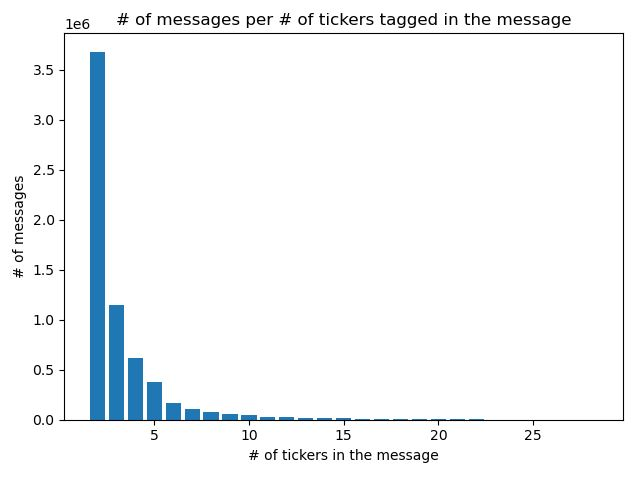
\includegraphics[width=0.75\textwidth]{hist_tic.JPG}
%    \caption{Histogram of the number of tickers per message, across all messages referring to more than one ticker. The maximum number of tickers per message amounts to 28 and corresponds to 11 messages in the sample.}
%    \label{fig:histtic}
%\end{figure}

%\begin{figure}[h]
%    \centering
%    \includegraphics[width=0.75\textwidth]{uniq.JPG}
%    \caption{Total number of messages with double counting (red) compared to the total number of messages without double counting (blue). Numbers are aggregated daily.}
%    \label{fig:uniq}
%\end{figure}

%\begin{figure}[h]
%    \centering
%    \includegraphics[width=0.75\textwidth]{ratio.JPG}
%    \caption{Ratio between the number of messages with double counting and the number of messages without double counting. Numbers are aggreaged daily.}
%    \label{fig:ratio}
%\end{figure}

%\newpage 


%\clearpage
\subsection{User Summary Statistics}\label{app_userstats}

Left plot of Figure \ref{fig:data-stocktwits1} shows a log-log histogram of the number of followers per user and a right plot shows a log-log histogram of the number of messages posted by users. There are a few users with many followers (they can be seen as ``influencers"), and many users with a few followers. In addition, most users seem to post on average between 10 and 400 messages and a few post a lot more. Overall, this appears to be a well balanced network structure. A more detailed study of the network effects on market sentiment is beyond the scope of this paper.



\begin{figure*}[h]
\centering
        \begin{subfigure}{0.49\textwidth}   
            \centering 
            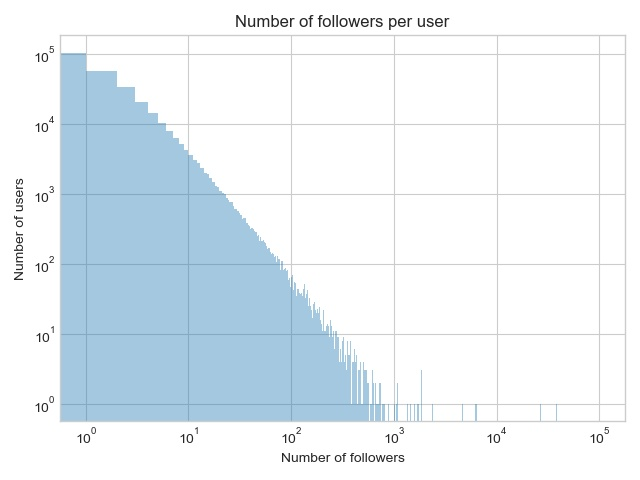
\includegraphics[width=\textwidth]{Followers.JPG}
        \end{subfigure}
        \begin{subfigure}{0.49\textwidth}
            \centering
            \includegraphics[width=\textwidth]{Tweets.jpg}
        \end{subfigure}

        \mycaption{User summary statistics}{Left graph is a log-log histogram of the number of followers per user and the right graph shows the log-log histogram of the number of messages posted by users.} 
        \label{fig:data-stocktwits1}
\end{figure*}



%\clearpage
\subsection{Anomalies} \label{app_ano}

We discuss here two anomalies that appear in the word clouds in Figure \ref{wordclouds}.

The term ``aldox'' in the bullish cloud caught our attention. After some research, it is an abbreviation for Aldoxorubicin, a drug against tumors and is associated with pharmaceutical messages where investors were very enthusiastic about it. An example of a related message is ``aldox is on the slide. have great faith this is truly world change". That is why the term is appearing almost exclusively in bullish messages, hence in the bullish cloud.

The bearish cloud contains the term "long position open", which seems like a bullish signal. Closer inspection shows that this term frequently appears in bearish user-labeled messages of intraday alerts such as ``sell \$labd close labd long position. open labd short position. time: 14:53 ny price: \$13.64 zquant intraday alerts''. However, this anomaly is not an issue. We tested what happened when "long position open" is fed as a message into our sentiment classifier. As a message, it consists of the trigram "long position open", the two bigrams ``long position'' and ``position open'', and the single words as unigrams. This results in a bullish score of 0.91 and the message is---correctly---classified as bullish. 




%\clearpage
\subsection{Coverage}\label{app_coverage}

Stocktwits is neither regulated nor moderated, so one needs to filter the information that we use. Even if Stocktwits has valuable information from respected contributors, a blog\footnote{\url{https://www.warriortrading.com/stocktwits-review}, last accessed on 1st of July 2022.} describes the concerns that may rise when using Stocktwits as a financial information provider, namely self-promotion, lack of credibility and other noise. To diversify noise and better extract information, we exclude from our sample tickers that are rarely discussed. Thereto, we compute the median of daily message volume for each ticker and exclude from our sample tickers with a median of less than 50. Decreasing the median threshold increases the coverage at the expense of more noise in the daily polarity. Figure \ref{fig:coverage} shows the coverage as a function of the median threshold. To increase the coverage we need to decrease the threshold a lot (e.g., decreasing the median threshold to 40 from 50 would increase the number of tickers covered to merely 22 from 19). We chose a median threshold of 50 as a balanced trade-off between noise and coverage. 

\begin{figure}[h]
    \centering
    \includegraphics[width=0.75\textwidth]{trim.JPG}
    \mycaption{Ticker coverage}{Coverage as a function of the median threshold. A lower threshold increases the coverage at the expense of a bigger bias in the polarity.}
    \label{fig:coverage}
\end{figure}

Table \ref{tab:listcov} shows the list of the 19 tickers above this threshold and their associated market capitalization as of 31st of December 2019. It appears that these most discussed tickers cover all sizes of stock, and hence we avoid big-firm bias. Also, it includes not only single firms but also ETFs on alternative investments. Finally, we cover several sectors so even if we have a restrictive universe, it is well diversified.

\begin{table}[h]
\centering
\begin{tabular}{l|l|c}
Ticker & Name                    & Market capitalization\\ \hline \hline
AAPL   & Apple                   & 1287\\
AMD    & Advanced Micro Devices  & 53 \\
AMRN   & Amarin                  & 7 \\
AMZN   & Amazon                  & 920 \\
BABA   & Alibaba                 & 571 \\
BAC    & Bank of America         & 311 \\
BB     & BlackBerry              & 4 \\
FB     & Facebook                & 585 \\
GLD    & Gold ETF                & 59 \\
IWM    & Small-Cap ETF           & 55 \\
JNUG   & Direxion                & 0.5 \\
MNKD   & MannKind Corporation    & 0.2 \\
NFLX   & Netflix                 & 142 \\
PLUG   & Plug Power              & 1 \\
QQQ    & Nasdaq100 ETF           & 134\\
SPY    & S\&P500 ETF             & 391 \\
TSLA   & Tesla                   & 76 \\
TWTR   & Twitter                 & 25 \\
UVXY   & VIX ETF                 & 0.8 \\
\end{tabular}
\mycaption{Ticker coverage}{Coverage after the trimming process. List of tickers and corresponding market capitalization as of 31st of December 2019.}
\label{tab:listcov}
\end{table}

%\input{ros.tex}






\clearpage
\subsection{Classifier Performance}\label{app_class}


We first recap the definition of the basic performance measures for a binary classifier. First, one has to choose one class as the positive class. Instances (messages) are then divided according to their predicted and actual labels into true positives TP (predicted positive, actual positive), false positives FP (predicted positive, actual negative), true negatives TN (predicted negative, actual negative), and false negatives FN (predicted negative, actual positive). Precision $PRE=\dfrac{TP}{TP+FP}$ is the proportion of true positives among the predicted positives. Recall $REC = \dfrac{TP}{TP+FN}$ is the proportion of true positives among the actual positives. The precision-recall trade-off is captured by the F1 score, $\dfrac{2 \cdot PRE \cdot REC}{PRE + REC}$, the harmonic mean of precision and recall.  

Tables \ref{classif-out} and \ref{classif-in} show the confusion matrices of our combined classifier out-of-sample and in-sample, respectively. We define accuracy as the fraction of correct predictions, omitting the messages with a predicted neutral sentiment. We thus obtain an out-of-sample accuracy of 85.9\%. The in-sample accuracy is 87.4\%. 
 

\begin{table}[H]
\centering
\begin{tabular}{cl|ll|}
\cline{3-4}
\multicolumn{1}{l}{}                        &         & \multicolumn{2}{c|}{True}               \\ \cline{3-4}
\multicolumn{1}{l}{}                        &         & \multicolumn{1}{l|}{Bullish} & Bearish  \\ \cline{1-4}
\multicolumn{1}{|c|}{\multirow{3}{*}{Predicted}} & Bullish & 3'555'896                      & 155'280   \\ \cline{2-2}
\multicolumn{1}{|c|}{}                      & Neutral & 663'541                       & 160'423    \\ \cline{2-2}
\multicolumn{1}{|c|}{}                      & Bearish & 550'928                       & 746'261  \\ \cline{1-4}
\end{tabular}
\mycaption{Confusion matrix for the combined classifier out-of-sample}{Rows are the predicted class of the combined classifier, columns are the user-labels. Values are the number of messages in the corresponding category.}
\label{classif-out}
\end{table}

\begin{table}[H]
\centering
\begin{tabular}{cl|ll|}
\cline{3-4}
\multicolumn{1}{l}{}                        &         & \multicolumn{2}{c|}{True}               \\ \cline{3-4}
\multicolumn{1}{l}{}                        &         & \multicolumn{1}{l|}{Bullish} & Bearish   \\ \cline{1-4}
\multicolumn{1}{|c|}{\multirow{3}{*}{Predicted}} & Bullish &  14'433'375                            & 532'509    \\ \cline{2-2}
\multicolumn{1}{|c|}{}                      & Neutral &  2'656'730                            &  642'329  \\ \cline{2-2}
\multicolumn{1}{|c|}{}                      & Bearish &  1'992'535                            &  3'071'837 \\ \cline{1-4}
\end{tabular}
\mycaption{Confusion matrix for the combined classifier in-sample}{Rows are the predicted class of the combined classifier, columns are the user-labels. Values are the number of messages in the corresponding category.}
\label{classif-in}
\end{table}


%Good comment to include
%When we think about, what is important in this classification exercise: a risk-averse investor would rather stay out of the market (i.e., realize zero return, no loss) rather than risking a false positive. (leading to a bad investment return, potential loss).
%So the more risk-averse the investor, the larger should be the precision.
%On the other hand, a risky profit seeking investor would regret having missed a good opportunity, i.e., false negative.
%So the risky profit seeking investor prefers a large recall.


 
 
%\clearpage
\subsection{Examples of Classified Messages}\label{app_exampleclass}

Here are some representative examples of classifications. Typical messages classified as bullish contain terms such as “buy buy” or “hope the pump come soon”. Whereas typical bearish messages contain terms such as “sell everything” or “start short position here”. Neutral messages are either empty, or irrelevant to finance (e.g., ``political posturing friend''\footnote{This is a reply to the message ``honestly, how dumb can you be to believe that china was going to buy significant amount of agricultural products after the breakdown in trade talks. Even if they buy it will be just a little bit and not significant''}), or ambiguous (e.g., “lol wow”).

%\clearpage
\subsection{Sentiment-Sorted Portfolios for Various Thresholds}\label{app_CAPport}
As the thresholds $U_t(x)$ and $L_t(x)$ are functions of the hyperparameter $x$, we provide for robustness check the results of our CAP-sorted portfolios for the values $x = 1.96$  (95\% confidence band) in Figure \ref{fig:pf1}, and for $x = 2.81$ (99.5\% confidence band) in Figure \ref{fig:pf3}. The portfolio performance arguably depends on the choice of $x$. In particular, the smaller $x$ the more likely the bearish portfolio exhibits positive returns. On the other hand, the larger $x$ the more likely the bullish portfolio misses the opportunities of positive returns. A careful gauging of $x$, possibly asymmetric in bullish and bearish, is therefore required for a real-world implementation of these strategies. Results could also improve for a larger cross-section of stocks than the 19 of our reduced sample.


%\begin{figure}[h]
%    \centering
%    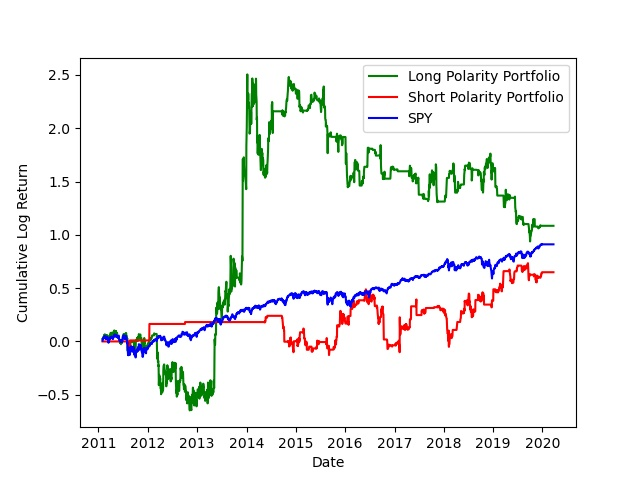
\includegraphics[width=0.5\textwidth]{cumulative_log_return1.jpg}
%    \caption{Cumulative log returns of bullish and bearish portfolios for $x=1.96$, and S\&P500.}
%    \label{fig:cumpf1}
%\end{figure}

\begin{figure*}[h]
        \centering
       %\begin{subfigure}[b]{0.42\textwidth}
       %    \centering
       %    \includegraphics[width=\textwidth]{boxplot1.jpg}
       %    \caption*{Distribution of returns}
       %\end{subfigure}
       %\quad
       %\begin{subfigure}[b]{0.42\textwidth}  
       %    \centering 
       %    \includegraphics[width=\textwidth]{boxplot_zoomed1.jpg}
       %    \caption*{Distribution of returns - zoomed}  
       %\end{subfigure}
       %\vskip\baselineskip
        \begin{subfigure}[b]{0.42\textwidth}   
            \centering 
    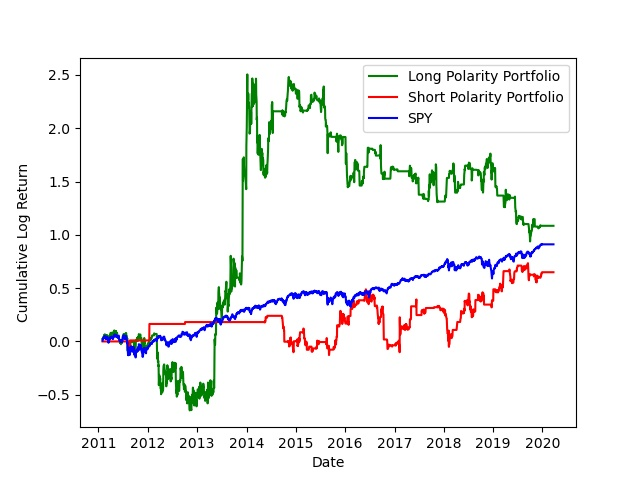
\includegraphics[width=\textwidth]{cumulative_log_return1.jpg}
    \caption*{Cumulative log returns}
        \end{subfigure}
        \quad
        \begin{subfigure}[b]{0.42\textwidth}   
            \centering 
            \includegraphics[width=\textwidth]{distribution_positions1.jpg}
            \caption*{Distribution of number of positions}   
        \end{subfigure}
                \vskip\baselineskip
        \begin{subfigure}[b]{0.42\textwidth}   
            \centering 
            \includegraphics[width=\textwidth]{positions1.jpg}
            \caption*{Number of positions over time}
        \end{subfigure}
        \quad
        \begin{subfigure}[b]{0.42\textwidth}   
            \centering 
            \includegraphics[width=\textwidth]{returns1.jpg}
            \caption*{Daily returns}  
        \end{subfigure}
        \mycaption{Bullish and bearish portfolios for $x = 1.96$}{Top left plot shows the cumulative log returns of the portfolios over the years, top right plot shows the distribution of the number of positions in the portfolios, bottom left plot is the number of positions over time and bottom right plot is the daily returns of both portfolios.}
        \label{fig:pf1}
    \end{figure*}

 
%\begin{figure}[h]
%    \centering
%    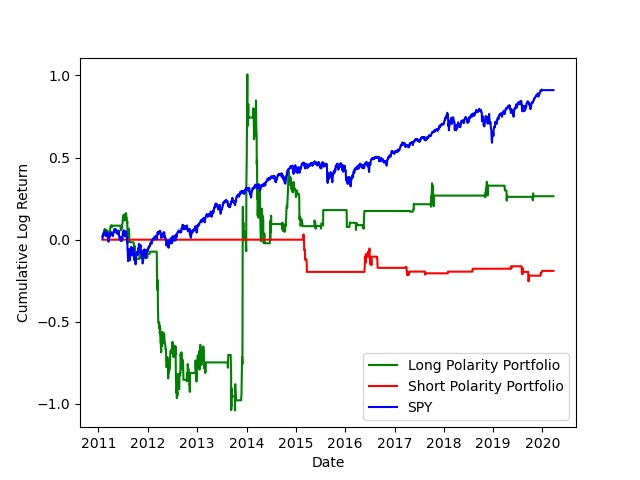
\includegraphics[width=0.5\textwidth]{cumulative_log_return3.jpg}
%    \caption{Cumulative log returns of bullish and bearish portfolios for $x=2.81$, and S\&P500.}
%    \label{fig:cumpf3}
%\end{figure}

\begin{figure*}[h]
        \centering
        %\begin{subfigure}[b]{0.42\textwidth}
        %    \centering
        %    \includegraphics[width=\textwidth]{boxplot3.jp%g}
        %    \caption*{Distribution of returns}
        %\end{subfigure}
        %\quad
        %\begin{subfigure}[b]{0.42\textwidth}  
        %    \centering 
        %    \includegraphics[width=\textwidth]{boxplot_zoo%med3.jpg}
        %    \caption*{Distribution of returns - zoomed}  
        %\end{subfigure}
        %\vskip\baselineskip
        \begin{subfigure}[b]{0.42\textwidth}   
            \centering 
        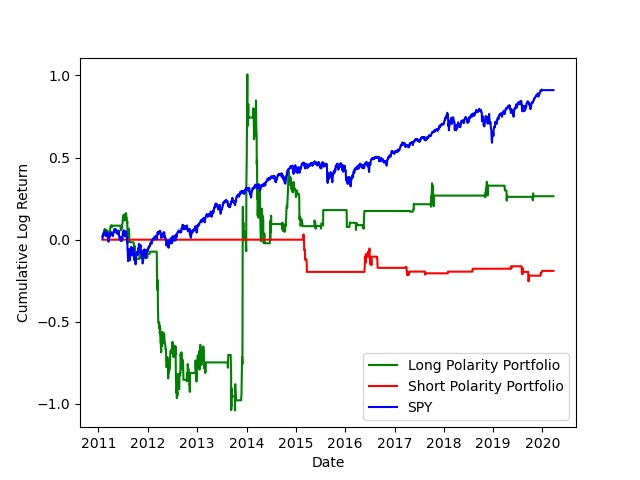
\includegraphics[width=\textwidth]{cumulative_log_return3.jpg}
        \caption*{Cumulative log returns}
        \end{subfigure}
        \quad
        \begin{subfigure}[b]{0.42\textwidth}   
            \centering 
            \includegraphics[width=\textwidth]{distribution_positions3.jpg}
            \caption*{Distribution of number of positions}   
        \end{subfigure}
                \vskip\baselineskip
        \begin{subfigure}[b]{0.42\textwidth}   
            \centering 
            \includegraphics[width=\textwidth]{positions3.jpg}
            \caption*{Number of positions over time}
        \end{subfigure}
        \quad
        \begin{subfigure}[b]{0.42\textwidth}   
            \centering 
            \includegraphics[width=\textwidth]{returns3.jpg}
            \caption*{Daily returns}  
        \end{subfigure}
        \mycaption{Bullish and bearish portfolios for $x=2.81$}{Top left plot shows the cumulative log returns of the portfolios over the years, top right plot shows the distribution of the number of positions in the portfolios, bottom left plot is the number of positions over time and bottom right plot is the daily returns of both portfolios.}
        \label{fig:pf3}
    \end{figure*}


% \newpage

% \subsection*{To discuss}

% \begin{figure}[H]
%     \centering
%     \includegraphics[width=0.75\textwidth]{opti_thresh_monday.JPG}
%     \caption{F1-score of long/not-long classifier in green, short/not-short classifier in red. Blue circles are optimal thresholds, maximizing F1 score. CAP is computed over the last 15 days and portfolio is rebalanced every Monday.}
%     \label{fig:my_label}
% \end{figure}

% \begin{table}[H]
% \centering
% \begin{tabular}{ll|lll|l}
% \cline{3-5}
%                               &       & \multicolumn{3}{c|}{event type}                                       &  \\ \cline{3-5}
%                               &       & \multicolumn{1}{l|}{bullish} & \multicolumn{1}{l|}{neutral} & bearish &  \\ \cline{1-5}
% \multicolumn{1}{|c|}{}         & long  & \multicolumn{1}{l|}{}      & \multicolumn{1}{l|}{20}      & 21      &  \\ \cline{2-5}
% \multicolumn{1}{|c|}{position} & none  & \multicolumn{1}{l|}{275}     & \multicolumn{1}{l|}{275}     & 252     &  \\ \cline{2-5}
% \multicolumn{1}{|l|}{}         & short & \multicolumn{1}{l|}{33}      & \multicolumn{1}{l|}{19}      & 88      &  \\ \cline{1-5}
% \end{tabular}
% \caption{Confusion matrix for the portfolio rebalanced every Monday. We build a long-short portfolio based on CAP over the last 15 days. Long-short positions are determined using optimal CAP thresholds, obtained by maximizing F1-Score of two distinct classifiers.}
% \end{table}

% \begin{figure}[H]
%     \centering
%     \includegraphics[width=0.75\textwidth]{opti_thresh_tuesday.JPG}
%     \caption{F1-score of long/not-long classifier in green, short/not-short classifier in red. Blue circles are optimal thresholds, maximizing F1 score. CAP is computed over the last 15 days and portfolio is rebalanced every Tuesday.}
%     \label{fig:my_label}
% \end{figure}

% \begin{table}[H]
% \centering
% \begin{tabular}{ll|lll|l}
% \cline{3-5}
%                               &       & \multicolumn{3}{c|}{event type}                                       &  \\ \cline{3-5}
%                               &       & \multicolumn{1}{l|}{bullish} & \multicolumn{1}{l|}{neutral} & bearish &  \\ \cline{1-5}
% \multicolumn{1}{|c|}{}         & long  & \multicolumn{1}{l|}{71}      & \multicolumn{1}{l|}{34}      & 13      &  \\ \cline{2-5}
% \multicolumn{1}{|c|}{position} & none  & \multicolumn{1}{l|}{304}     & \multicolumn{1}{l|}{296}     & 278     &  \\ \cline{2-5}
% \multicolumn{1}{|l|}{}         & short & \multicolumn{1}{l|}{21}      & \multicolumn{1}{l|}{36}      & 70      &  \\ \cline{1-5}
% \end{tabular}
% \caption{Confusion matrix for the portfolio rebalanced every Tuesday. We build a long-short portfolio based on CAP over the last 15 days. Long-short positions are determined using optimal CAP thresholds, obtained by maximizing F1-Score of two distinct classifiers.}
% \end{table}

% \begin{figure}[H]
%     \centering
%     \includegraphics[width=0.75\textwidth]{opti_thresh_wednesday.JPG}
%     \caption{F1-score of long/not-long classifier in green, short/not-short classifier in red. Blue circles are optimal thresholds, maximizing F1 score. CAP is computed over the last 15 days and portfolio is rebalanced every Wednesday.}
%     \label{fig:my_label}
% \end{figure}


% \begin{table}[H]
% \centering
% \begin{tabular}{ll|lll|l}
% \cline{3-5}
%                               &       & \multicolumn{3}{c|}{event type}                                       &  \\ \cline{3-5}
%                               &       & \multicolumn{1}{l|}{bullish} & \multicolumn{1}{l|}{neutral} & bearish &  \\ \cline{1-5}
% \multicolumn{1}{|c|}{}         & long  & \multicolumn{1}{l|}{88}      & \multicolumn{1}{l|}{50}      & 21      &  \\ \cline{2-5}
% \multicolumn{1}{|c|}{position} & none  & \multicolumn{1}{l|}{296}     & \multicolumn{1}{l|}{299}     & 281     &  \\ \cline{2-5}
% \multicolumn{1}{|l|}{}         & short & \multicolumn{1}{l|}{20}      & \multicolumn{1}{l|}{17}      & 59      &  \\ \cline{1-5}
% \end{tabular}
% \caption{Confusion matrix for the portfolio rebalanced every Wednesday. We build a long-short portfolio based on CAP over the last 15 days. Long-short positions are determined using optimal CAP thresholds, obtained by maximizing F1-Score of two distinct classifiers.}
% \end{table}

% \begin{figure}[H]
%     \centering
%     \includegraphics[width=0.75\textwidth]{opti_thresh_thursday.JPG}
%     \caption{F1-score of long/not-long classifier in green, short/not-short classifier in red. Blue circles are optimal thresholds, maximizing F1 score. CAP is computed over the last 15 days and portfolio is rebalanced every Thursday.}
%     \label{fig:my_label}
% \end{figure}


% \begin{table}[H]
% \centering
% \begin{tabular}{ll|lll|l}
% \cline{3-5}
%                               &       & \multicolumn{3}{c|}{event type}                                       &  \\ \cline{3-5}
%                               &       & \multicolumn{1}{l|}{bullish} & \multicolumn{1}{l|}{neutral} & bearish &  \\ \cline{1-5}
% \multicolumn{1}{|c|}{}         & long  & \multicolumn{1}{l|}{188}     & \multicolumn{1}{l|}{123}     & 73      &  \\ \cline{2-5}
% \multicolumn{1}{|c|}{position} & none  & \multicolumn{1}{l|}{196}     & \multicolumn{1}{l|}{223}     & 228     &  \\ \cline{2-5}
% \multicolumn{1}{|l|}{}         & short & \multicolumn{1}{l|}{20}      & \multicolumn{1}{l|}{20}      & 60      &  \\ \cline{1-5}
% \end{tabular}
% \caption{Confusion matrix for the portfolio rebalanced every Thursday. We build a long-short portfolio based on CAP over the last 15 days. Long-short positions are determined using optimal CAP thresholds, obtained by maximizing F1-Score of two distinct classifiers.}
% \end{table}


% \begin{figure}[H]
%     \centering
%     \includegraphics[width=0.75\textwidth]{opti_thresh_friday.JPG}
%     \caption{F1-score of long/not-long classifier in green, short/not-short classifier in red. Blue circles are optimal thresholds, maximizing F1 score. CAP is computed over the last 15 days and portfolio is rebalanced every Friday.}
%     \label{fig:my_label}
% \end{figure}


% \begin{table}[H]
% \centering
% \begin{tabular}{ll|lll|l}
% \cline{3-5}
%                               &       & \multicolumn{3}{c|}{event type}                                       &  \\ \cline{3-5}
%                               &       & \multicolumn{1}{l|}{bullish} & \multicolumn{1}{l|}{neutral} & bearish &  \\ \cline{1-5}
% \multicolumn{1}{|c|}{}         & long  & \multicolumn{1}{l|}{94}      & \multicolumn{1}{l|}{43}      & 21      &  \\ \cline{2-5}
% \multicolumn{1}{|c|}{position} & none  & \multicolumn{1}{l|}{284}     & \multicolumn{1}{l|}{283}     & 263     &  \\ \cline{2-5}
% \multicolumn{1}{|l|}{}         & short & \multicolumn{1}{l|}{26}      & \multicolumn{1}{l|}{40}      & 77      &  \\ \cline{1-5}
% \end{tabular}
% \caption{Confusion matrix for the portfolio rebalanced every Friday. We build a long-short portfolio based on CAP over the last 15 days. Long-short positions are determined using optimal CAP thresholds, obtained by maximizing F1-Score of two distinct classifiers.}
% \end{table}


%\begin{figure}
%    \centering
%    \includegraphics[width=\textwidth]{marketvol_relchange.JPG}
%    \caption{Caption}
%    \label{fig:my_label}
%\end{figure}
%
%\begin{figure}
%    \centering
%    \includegraphics[width=\textwidth]{aapl_vol_relchange.JPG}
%    \caption{Caption}
%    \label{fig:my_label}
%\end{figure}
%
%\begin{figure}
%    \centering
%    \includegraphics[width=\textwidth]{rel_activity_volume.JPG}
%    \caption{Caption}
%    \label{fig:my_label}
%\end{figure}










